% Umístění obsahu paměťového média do příloh je vhodné konzultovat s vedoucím
%\chapter{Obsah přiloženého paměťového média}

%\chapter{Manuál}

%\chapter{Konfigurační soubor}

%\chapter{RelaxNG Schéma konfiguračního souboru}

%\chapter{Plakát}

\chapter{Seznam použitých dílů}
\label{usedparts}

\begin{table}[hbt]
\centering
\caption{Použité díly a jejich nákupní cena}
\begin{tabular}{| p{0.65\linewidth}|c|c|}
\hline
Název komponenty & Počet kusů & Cena celkem \\ & & \\ \hline
ESP32 vývojová deska  & 1 & \$4,30 \\ \hline
XL4016 nastavitelný DC-DC step down regulátor napětí 8A 200W & 1 & \$2,74 \\ \hline
Servo 9g SG90 & 18 & \$19,25 \\ \hline
TENSTAR ROBOT I2C 16 kanálový 12-bit PWM/Servo Driver PCA9685 & 1 & \$2,04 \\ \hline
3,7V 4000mAh 104080 LiPol baterie & 2 & \$16,98 \\ \hline
Sada distančních sloupků, šroubů a matic & 1 & \$3,95 \\ \hline
Sada pinů a dutinek & 1 & \$1,88 \\ \hline
Stahovací bužírky, konektory, drátky a pájivá pole & \-- & \textasciitilde\$6 \\ \hline
Cena celkem & \-- & \textasciitilde\$60 \\ \hline
\end{tabular}
\end{table}


\chapter{Schéma zapojení elektroniky}
\label{schematics}

\begin{figure}[hbt]
	\centering
	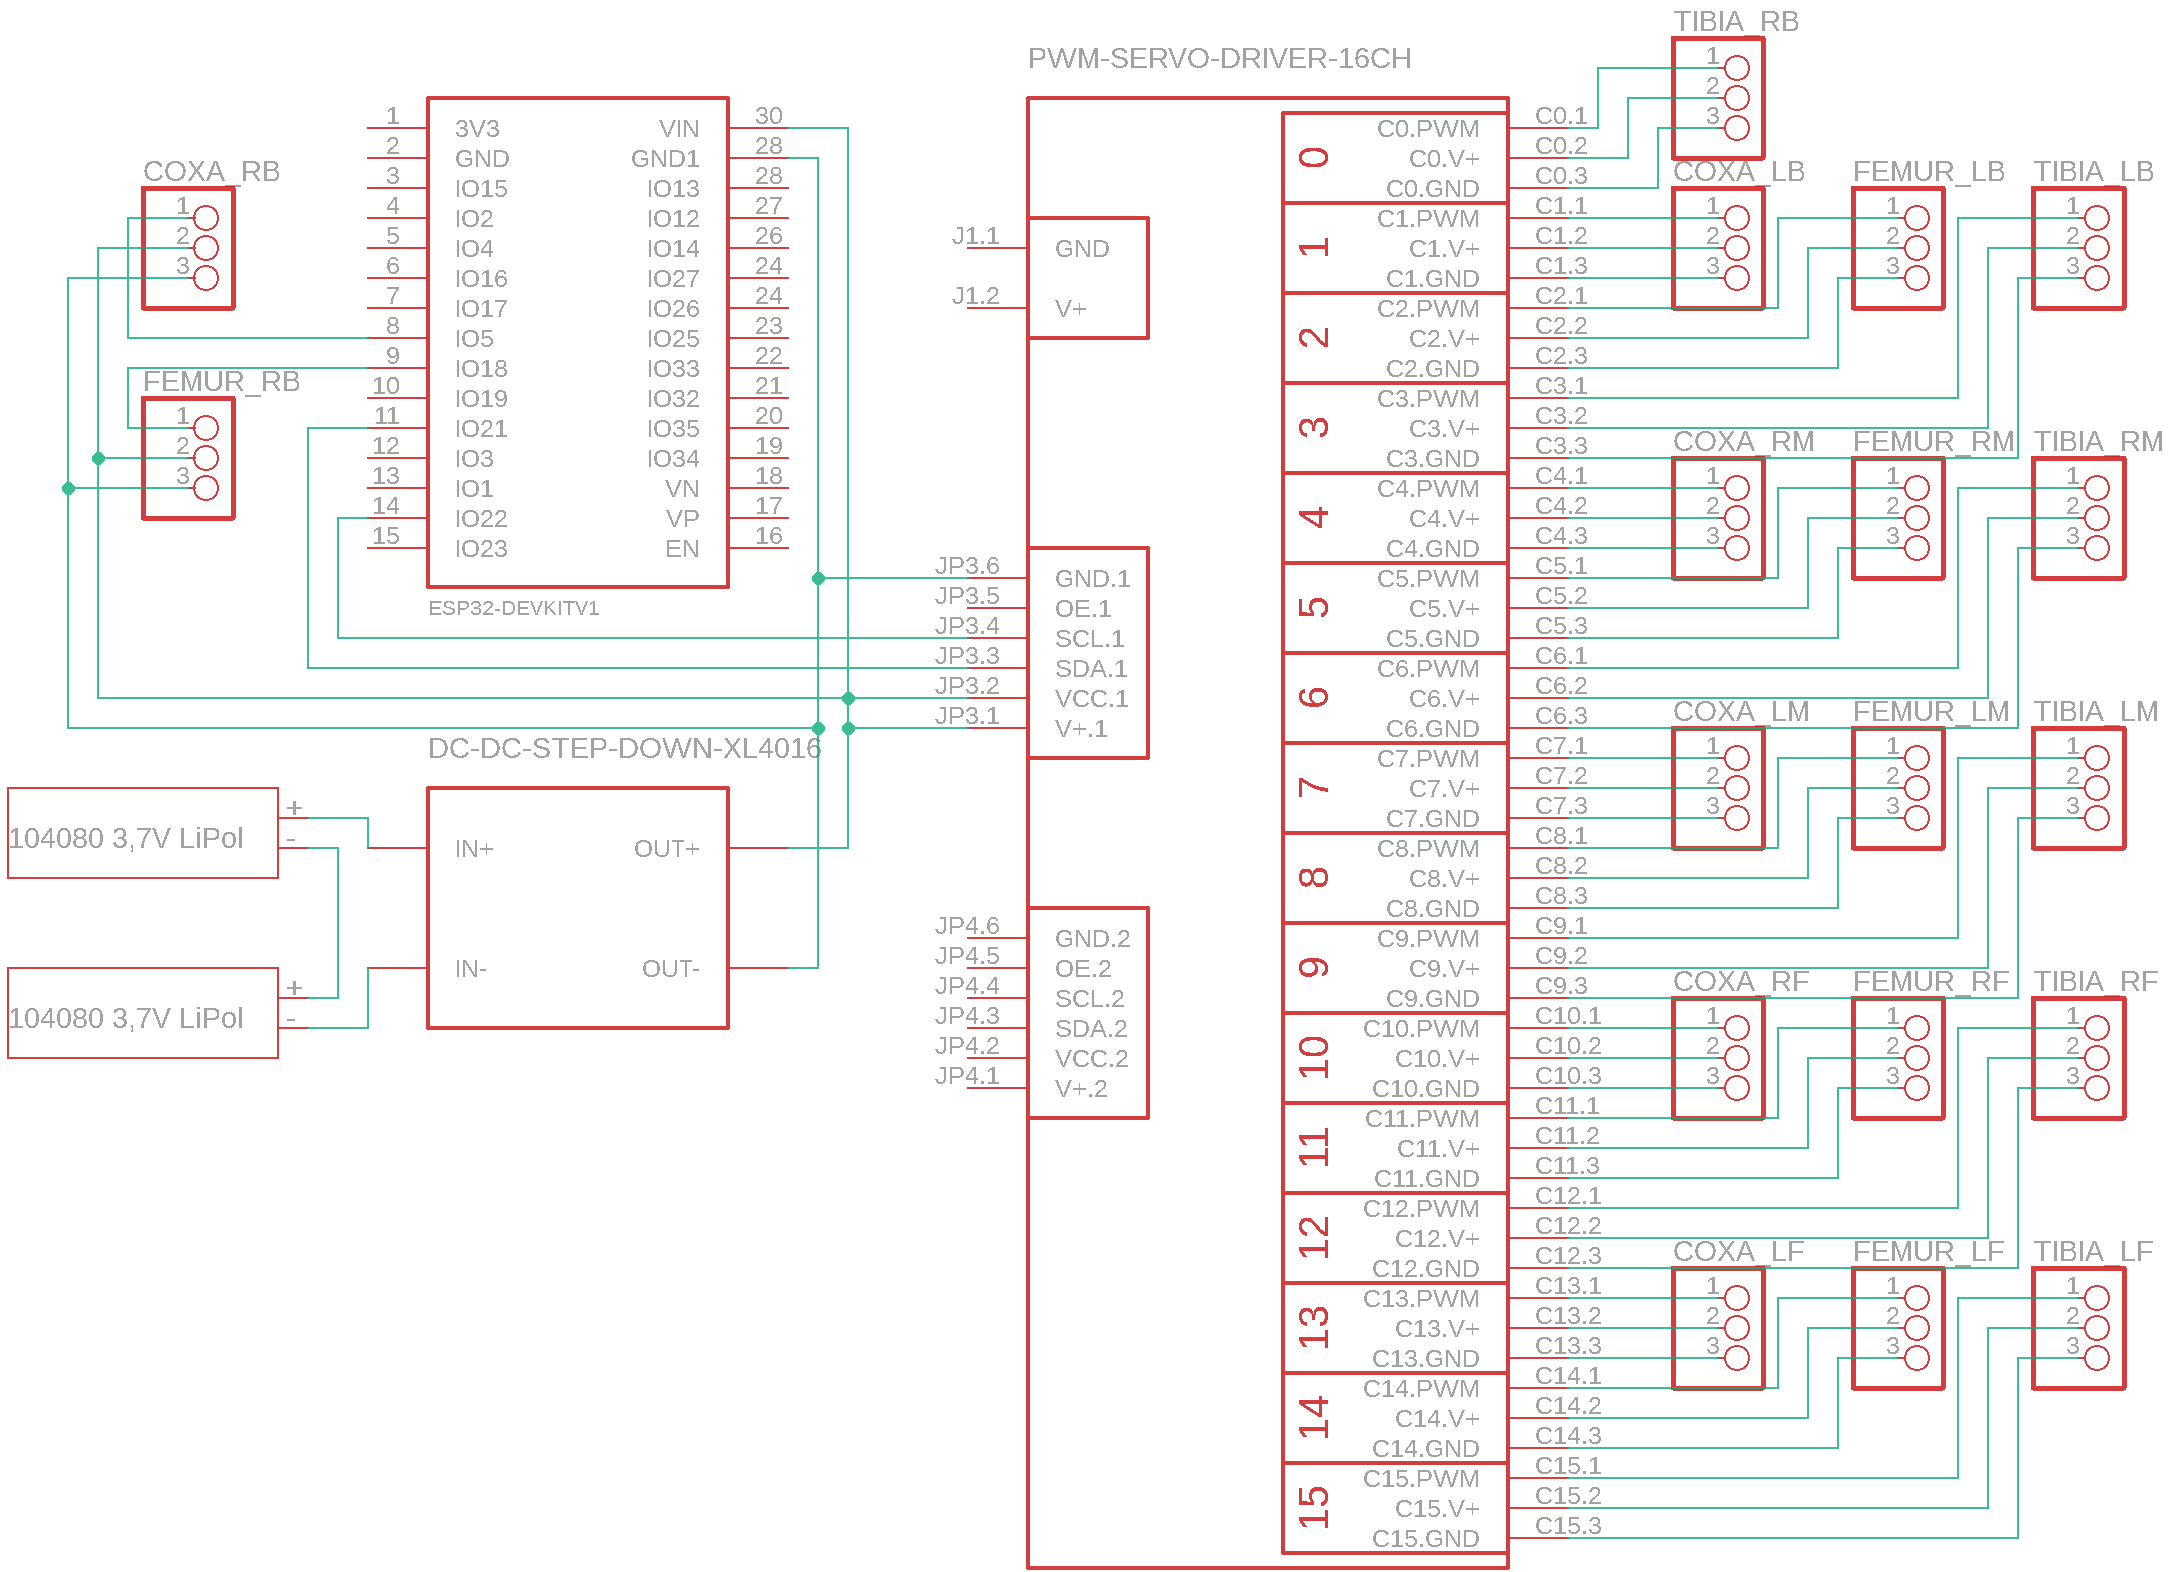
\includegraphics[width=1\textwidth, angle=90, origin=c]{obrazky-figures/schematics.png}
	\caption{Schéma zapojení elektroniky}
    \label{schem}
\end{figure}
